% ------------------------------------------------------------------------------
% QUESTION A : Esquisse des modes de vibration
% ------------------------------------------------------------------------------
\subsubsection*{Question a) Allure générale des modes de vibration}

\begin{itemize}
    \item \textbf{Deuxième mode de la corde ($n = 2$, deux extrémités fixes) :} 
    La corde présente un nœud à chaque extrémité ainsi qu'un nœud central (soit 3 nœuds au total) et 2 ventres de vibration.
    
    \item \textbf{Troisième mode du tuyau fermé-ouvert ($n = 3$) :} 
    Pour un tuyau fermé à une extrémité et ouvert à l'autre, seuls les harmoniques impairs ($1, 3, 5, \dots$) existent. Le 3\textsuperscript{e} mode correspond au 5\textsuperscript{e} harmonique ($m = 5$). Il comporte un nœud à l'extrémité fermée et un ventre à l'extrémité ouverte, pour un total de 3 nœuds et 3 ventres.
\end{itemize}

\begin{center}
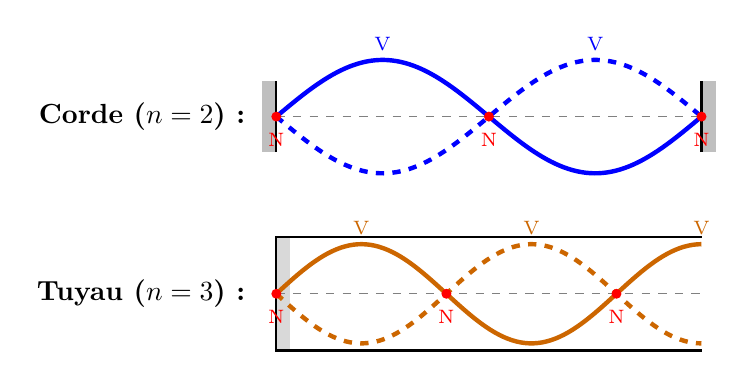
\begin{tikzpicture}[scale=0.9]
    % --- CORDE DE CONTREBASSE ---
    \begin{scope}[shift={(0,0)}]
        \node[anchor=east] at (-0.3,0) {\textbf{Corde ($n=2$) :}};
        % Extrémités fixes
        \fill[gray!50] (-0.2,-0.5) rectangle (0,0.5);
        \draw[thick] (0,-0.5) -- (0,0.5);
        \fill[gray!50] (6,-0.5) rectangle (6.2,0.5);
        \draw[thick] (6,-0.5) -- (6,0.5);
        % Axe
        \draw[dashed, gray] (0,0) -- (6,0);
        % Enveloppe du mode 2
        \draw[ultra thick, blue, domain=0:6, samples=100] plot (\x, {0.8*sin(2*180*\x/6)});
        \draw[ultra thick, blue, dashed, domain=0:6, samples=100] plot (\x, {-0.8*sin(2*180*\x/6)});
        % Nœuds et Ventres
        \foreach \x in {0, 3, 6} \fill[red] (\x,0) circle (2pt);
        \node[below, red, font=\scriptsize] at (0,-0.1) {N};
        \node[below, red, font=\scriptsize] at (3,-0.1) {N};
        \node[below, red, font=\scriptsize] at (6,-0.1) {N};
        \node[above, blue, font=\scriptsize] at (1.5,0.8) {V};
        \node[above, blue, font=\scriptsize] at (4.5,0.8) {V};
    \end{scope}

    % --- TUYAU ORGUE FERMÉ-OUVERT ---
    \begin{scope}[shift={(0,-2.5)}]
        \node[anchor=east] at (-0.3,0) {\textbf{Tuyau ($n=3$) :}};
        % Tuyau (Parois)
        \fill[gray!30] (0,-0.8) rectangle (0.2,0.8);
        \draw[thick] (0.2,0.8) -- (0,0.8) -- (0,-0.8) -- (0.2,-0.8);
        \draw[thick] (0,0.8) -- (6,0.8);
        \draw[thick] (0,-0.8) -- (6,-0.8);
        % Axe
        \draw[dashed, gray] (0,0) -- (6,0);
        % Ondes (5e harmonique : 2.5 quart d'onde sur L)
        \draw[ultra thick, orange!80!black, domain=0:6, samples=100] plot (\x, {0.7*sin(2.5*180*\x/6)});
        \draw[ultra thick, orange!80!black, dashed, domain=0:6, samples=100] plot (\x, {-0.7*sin(2.5*180*\x/6)});
        % Nœuds et Ventres
        \fill[red] (0,0) circle (2pt);
        \fill[red] (2.4,0) circle (2pt);
        \fill[red] (4.8,0) circle (2pt);
        \node[below, red, font=\scriptsize] at (0,-0.1) {N};
        \node[below, red, font=\scriptsize] at (2.4,-0.1) {N};
        \node[below, red, font=\scriptsize] at (4.8,-0.1) {N};
        \node[above, orange!80!black, font=\scriptsize] at (1.2,0.7) {V};
        \node[above, orange!80!black, font=\scriptsize] at (3.6,0.7) {V};
        \node[above, orange!80!black, font=\scriptsize] at (6,0.7) {V};
    \end{scope}
\end{tikzpicture}
\end{center}


% ------------------------------------------------------------------------------
% QUESTION B : Tension sur la corde
% ------------------------------------------------------------------------------
\subsubsection*{Question b) Calcul de la tension sur la corde de contrebasse}

\begin{enumerate}[label=\arabic*)]
    \item \textbf{Variables connues et recherchées :}
    \begin{itemize}[label= -]
        \item Longueur de la corde : $L_c = \qty{\CordeLongueur}{cm} = \qty{\fpeval{\CordeLongueur/100}}{m}$
        \item Masse linéique de la corde : $\mu = \qty{\CordeMasseLin}{kg/m}$
        \item Longueur du tuyau : $L_p = \qty{\TuyauLongueur}{cm} = \qty{\fpeval{\TuyauLongueur/100}}{m}$
        \item Vitesse du son dans l'air : $v_{\text{son}} = \qty{\CordeVitesseSon}{m/s}$
        \item Mode de la corde : $n_c = 2$ ($2^\text{e}$ harmonique)
        \item Mode du tuyau fermé-ouvert : $n_p = 3$ ($5^\text{e}$ harmonique)
        \item Variable recherchée : Tension dans la corde $T \text{ (N)}$
    \end{itemize}

    \item \textbf{Équations pertinentes :}
    \begin{itemize}[label= -]
        \item Fréquence du $3^\text{e}$ mode du tuyau fermé-ouvert ($5^\text{e}$ harmonique) :
        \[
        f_{p, 3} = \frac{5 v_{\text{son}}}{4 L_p}
        \]
        \item Fréquence du $2^\text{e}$ mode de la corde ($2^\text{e}$ harmonique) :
        \[
        f_{c, 2} = \frac{2 v_c}{2 L_c} = \frac{v_c}{L_c} \quad \text{avec} \quad v_c = \sqrt{\frac{T}{\mu}}
        \]
    \end{itemize}

    \item \textbf{Condition de résonance et isolation de $T$ :}
    Puisque les deux fréquences sont égales ($f_{c, 2} = f_{p, 3}$) :
    \[
    \frac{1}{L_c} \sqrt{\frac{T}{\mu}} = \frac{5 v_{\text{son}}}{4 L_p} \quad \implies \quad \sqrt{\frac{T}{\mu}} = \frac{5 L_c v_{\text{son}}}{4 L_p}
    \]
    En élevant au carré et en isolant la tension $T$ :
    \[
    T = \mu \cdot \left( \frac{5 L_c \cdot v_{\text{son}}}{4 L_p} \right)^2
    \]

    \item \textbf{Résolution numérique :}
    \[
    v_c = \frac{5 \cdot (\fpeval{\CordeLongueur/100}) \cdot \CordeVitesseSon}{4 \cdot (\fpeval{\TuyauLongueur/100})} = \qty{\fpeval{round((5 * \CordeLongueur * \CordeVitesseSon) / (4 * \TuyauLongueur), 2)}}{m/s}
    \]
    \[
    T = \CordeMasseLin \cdot \left( \fpeval{round((5 * \CordeLongueur * \CordeVitesseSon) / (4 * \TuyauLongueur), 4)} \right)^2 = \qty{\fpeval{round(\CordeMasseLin * ((5 * \CordeLongueur * \CordeVitesseSon) / (4 * \TuyauLongueur))^2, 2)}}{N}
    \]

    \item \textbf{Réponse :}
    La tension appliquée sur la corde de contrebasse est de \textbf{\qty{\fpeval{round(\CordeMasseLin * ((5 * \CordeLongueur * \CordeVitesseSon) / (4 * \TuyauLongueur))^2, 1)}}{N}}.
\end{enumerate}


% ------------------------------------------------------------------------------
% QUESTION C : Fréquence et longueur d'onde dans l'air
% ------------------------------------------------------------------------------
\subsubsection*{Question c) Fréquence et longueur d'onde des ondes sonores dans la pièce}

\begin{enumerate}[label=\arabic*)]
    \item \textbf{Variables connues et recherchées :}
    \begin{itemize}[label= -]
        \item Vitesse du son dans la pièce : $v_{\text{son}} = \qty{\CordeVitesseSon}{m/s}$
        \item Longueur du tuyau : $L_p = \qty{\fpeval{\TuyauLongueur/100}}{m}$
        \item Variables recherchées : Fréquence $f_{\text{son}} \text{ (Hz)}$ et longueur d'onde $\lambda_{\text{son}} \text{ (m)}$
    \end{itemize}

    \item \textbf{Équations pertinentes :}
    Lorsqu'une corde vibre, elle impose sa fréquence de vibration à l'air ambiant. Ainsi, la fréquence du son perçu est égale à la fréquence de vibration de la corde (et du tuyau) :
    \[
    f_{\text{son}} = f_{c, 2} = f_{p, 3} = \frac{5 v_{\text{son}}}{4 L_p}
    \]
    La longueur d'onde de ce son dans l'air dépend de la vitesse du son dans la pièce :
    \[
    \lambda_{\text{son}} = \frac{v_{\text{son}}}{f_{\text{son}}} = \frac{4 L_p}{5}
    \]

    \item \textbf{Résolution numérique :}
    \begin{itemize}[label= -]
        \item \textbf{Fréquence du son :}
        \[
        f_{\text{son}} = \frac{5 \cdot \CordeVitesseSon}{4 \cdot (\fpeval{\TuyauLongueur/100})} = \qty{\fpeval{round((5 * \CordeVitesseSon) / (4 * (\TuyauLongueur / 100)), 2)}}{Hz}
        \]
        \item \textbf{Longueur d'onde du son :}
        \[
        \lambda_{\text{son}} = \frac{4 L_p}{5} = \frac{4 \cdot (\fpeval{\TuyauLongueur/100})}{5} = \qty{\fpeval{round((4 * (\TuyauLongueur / 100)) / 5, 4)}}{m}
        \]
    \end{itemize}

    \item \textbf{Réponse :}
    Dans l'air ambiant de la pièce, l'onde sonore perçue a une fréquence de \textbf{\qty{\fpeval{round((5 * \CordeVitesseSon) / (4 * (\TuyauLongueur / 100)), 1)}}{Hz}} et une longueur d'onde de \textbf{\qty{\fpeval{round((4 * (\TuyauLongueur / 100)) / 5, 3)}}{m}} (soit \textbf{\qty{\fpeval{round(((4 * (\TuyauLongueur / 100)) / 5) * 100, 1)}}{cm}}).
\end{enumerate}